% Appendix 9: Zero Lines and Their Curvature
% Source pages: 281–284

\chapter{Zero Lines and Their Curvature}

\srcpage{281}

In Appendix~6 the concept of zero lines was introduced as lines that undergo no lateral
shifts in the transition from the linear-perspective system to the perceptual-perspective
system.  From a consideration of Ill.\,99 and~100 it is easy to see that in those cases
a vertical through the principal point of the picture was chosen as the zero line.  This
choice is fully justified: when depicting space from a single viewpoint, one must rely on
a single zero line, and this line should be as far as possible in the central part of the
picture, since this is how the artist ``on average'' paints the picture and how the viewer
contemplates it.

Let us examine the question of what the geometry of the depicted portion of space will be
under the corrective transfer of the artist's gaze.  For the zero line that is actually
realised in perception always corresponds to the central part of the visual field, so that
on transferring the gaze from one direction to another, the zero line changes accordingly.

Suppose the artist is observing some line that he takes as the zero line.  Suppose further
that this line is observed in foreshortening, as shown in Fig.\,9.1.  In the diagram,
line~$AA$ corresponds to the base of the picture, and line~$BB$ to the horizon in the
linear perspective system.  Line $AB$ is the image of the zero line under consideration
in the linear perspective system.  Since this line must undergo no lateral shifts in the
transition to the perceptual perspective system, the zero line in the latter can be
obtained from~$AB$ by vertical displacements of its points.  These displacements are of
different magnitude depending on which segment is taken as the unit of length.  Take as
the unit module the horizontal segment parallel to the picture plane, and consider three
cases: this segment lies in the picture plane ($l = 0$), at some distance from it
($l = l^*$), and in the region of the horizon ($l \to \infty$).  On Fig.\,9.1 these three
characteristic distances from the observer correspond to points $A$, $C$, and $B$.

\srcpage{282}

If the construction of the zero line begins from point~$A$, this means conveying the
nearest ground correctly and then constructing the further course of the zero line to the
scale of this ground.  Starting from point~$B$ means working in the opposite direction
and constructing the entire picture to the scale of the far ground; point~$C$ gives an
intermediate case.  This is of course only a logical scheme, not a description of actual
drawing technique.

These constructions are carried out by the formula
\begin{equation}
  \tilde{y}_2 = \frac{P_3(l)}{P_1(l_*)}+\left[y_1-\frac{P_3(l^*)}{P_1(l_*)}{}, \right] \tag{9.1}
\end{equation}
where $\tilde{y}_2$ is the $y_2$-coordinate brought to the chosen scale corresponding to
$l_* = l^*$, the functions $P_3$ and $P_2$ are defined in the preceding Appendix, and
$y_1(l_*)$ is the linear-perspective ordinate of the zero-line at the reference depth.
The written expression shows that at $l = l^*$ one has $\tilde{y}_2 = y_1(l^*)$, i.e.\
the linear and perceptual ordinates coincide at the reference point, facilitating comparison
of different variants of zero-line images.

\begin{figure}[H]
    \centering
    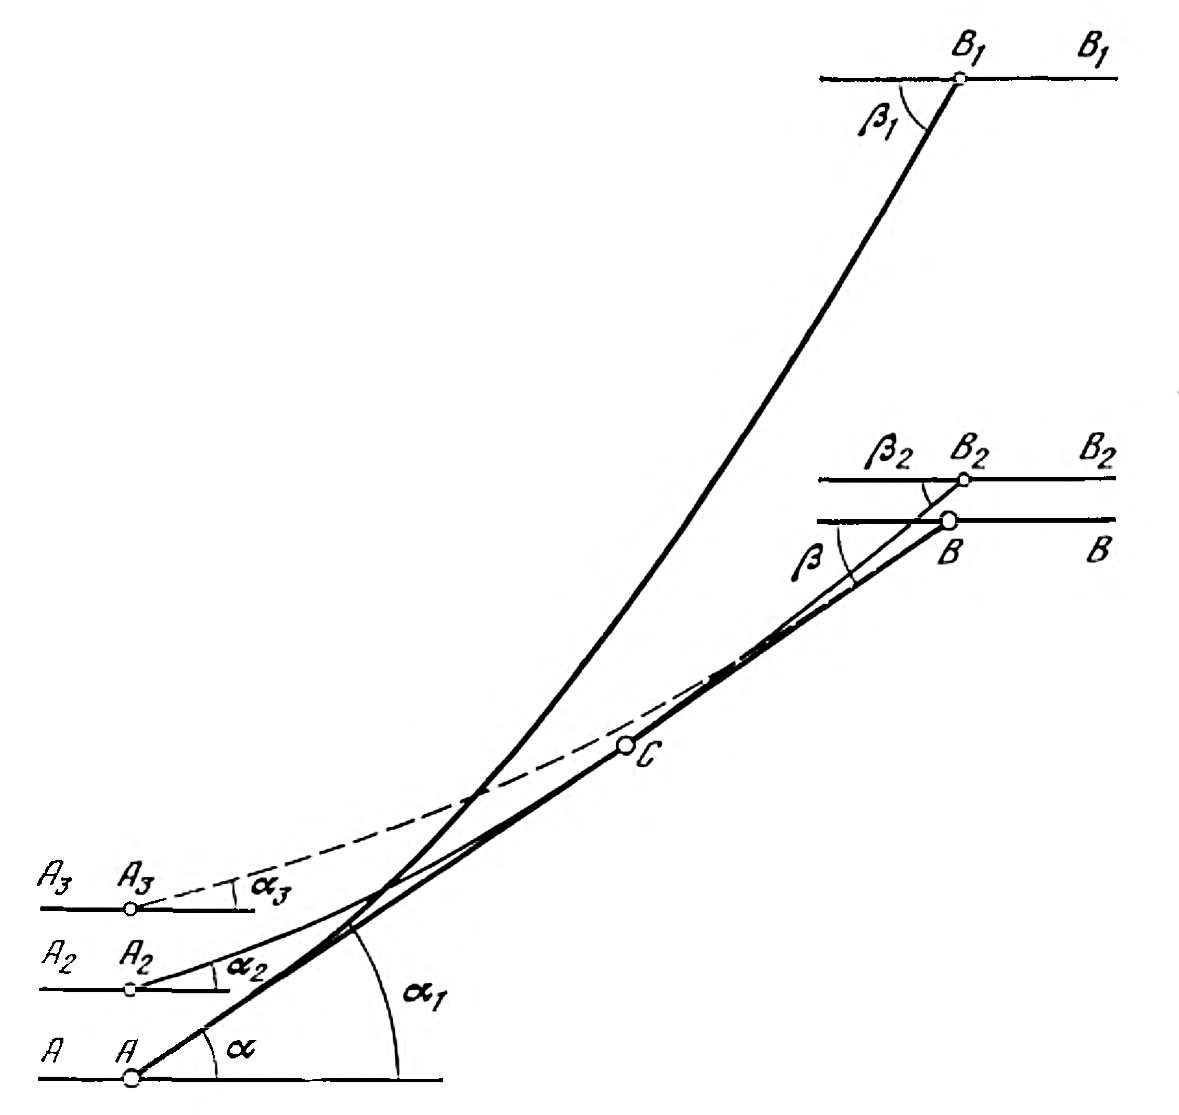
\includegraphics[width=0.85\linewidth]{figures/f9.1.png}
\end{figure}
\figblock{9.1}{Three variants of the zero-line image in perceptual perspective, depending
  on the reference depth~$l^*$.  Curve~$AB_1$ ($l^* = 0$): correct near ground but
  incorrect horizon angle.  Curve~$A_3B$ ($l^* \to \infty$): correct horizon angle but
  incorrect near-ground intersection.  Curve~$A_2B_2$ ($l^* = l^*$, intermediate):
  best compromise.  All curves are convex downward.}

Begin with the case $l^* = 0$.  Here the stretchings due to the size-constancy mechanism
yield the zero line as a curve~$AB_1$.  The angle~$\alpha_1$ of inclination of the zero
line to the picture base is unchanged compared with angle~$\alpha$ of the linear
perspective ($\alpha_1 = \alpha$).  It is important to note that both~$\alpha$ and the
appearance of downward convexity in the zero line fully correspond to visual perception,
as will be confirmed experimentally at the end of this Appendix.  However, if the zero
line is continued, the region near the horizon around point~$B_1$ will be distorted: the
angle between any line in the region of the horizon and the horizon line is always seen
exactly as in linear perspective, i.e.\ in the present case it should appear equal to~$\beta$,
whereas it turns out to be depicted as angle~$\beta_1 \neq \beta$.

\srcpage{283}

To avoid this, if one starts the construction from point~$B$, the horizon region is
depicted correctly, but in the near foreground the intersection of the new zero-line image
$A_3B$ with the lower edge of the picture~$A_3A_3$ occurs at angle~$\alpha_3 < \alpha$,
which contradicts visual perception.

Consequently, a perfect image of the zero line, taking into account not only linear
quantities but also angles, is excluded.  In this connection it may turn out that ``on
average'' the zero line is best transmitted if the starting point is~$C$ (curve~$A_2B_2$).
The angles of intersection of this curve with the lower edge~$A_2A_2$ ($\alpha_2$) and
with the horizon~$B_2B_2$ ($\beta_2$), although not corresponding to the visible angles
($\alpha_2 \neq \alpha$, $\beta_2 \neq \beta$), differ from them less than $\alpha_3$
and $\beta_1$ respectively.

\begin{figure}[H]
    \centering
    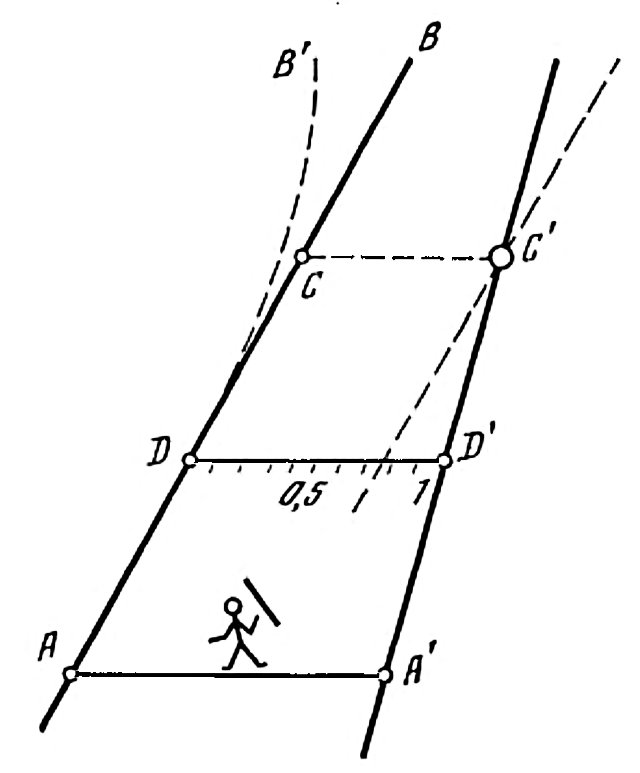
\includegraphics[width=0.45\linewidth]{figures/f9.2.png}
\end{figure}
\figblock{9.2}{Scheme of the experiment for measuring the curvature of a zero line
  observed in foreshortening.  The observer stands at the midpoint of strip~$AA_1$.
  Two readings of the ruler (aligned through~$C$, parallel first to~$OC$ and then to~$CB$)
  are compared; a difference indicates that the straight line~$OB$ of objective space is
  perceived as a curve in perceptual space.}

The actual curvature of zero lines observed in foreshortening can easily be registered
experimentally.  Fig.\,9.2 shows the scheme of the experiment.  The observer stands at the
midpoint of strip~$AA_1$.  The distance $AH = l_0$, and line~$OO'$ is graduated in
fractions of its length.  Object~$C$ is placed at the indicated position.  The ruler used
for sighting is held so that its trace on the ground appears to contain point~$C'$ and to
be parallel to the left side~$AB$ of the strip.  As can be seen, the experimental method
is the same as that described in Appendix~3.  The sole feature of the method is that
\emph{two} readings are taken: in the first, the ruler is held so that its trace on the
ground is parallel to~$OC$; in the second, so that it is parallel to~$CB$.  If the
straight line~$OB$ of perceptual space remains a straight line, there is no difference
between the first and second readings.  As experiment shows (conditions the same as those
described in Appendix~3 for $l_0 = 2$\,m), the first reading gives~0.765 and the second
0.866 (mean values from multiple readings by four observers at $l = 1$).  Consequently,
the objectively straight line~$OB$ turns out to be a curve in visual perception, shown
conventionally by the dashed curve~$OB'$.
